\subsection[Subsection]{Conceituação}
\begin{frame}
	\frametitle{Conceituação}
	Um sistema de \emph{License Plate Recognition} (\textbf{LPR}) 
	consiste em um \emph{hardware} e um \emph{software}
	integrados com o objetivo de reconhecer placas de veículos 
	a partir de imagens \cite{Anagnostopoulos2014}.

	\vspace{1em}

	Ou seja, o sistema recebe uma imagem e
	retorna o conteúdo da placa, se ela existir:

	\vspace{1em}
	
	\begin{center}	
	\begin{tikzpicture}
		\node[inner sep=0pt,outer sep=0pt] at (0,0) {\fbox{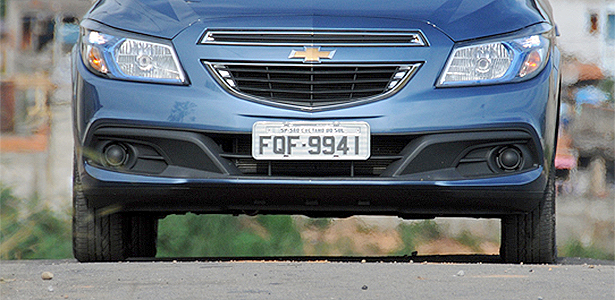
\includegraphics[width=4cm,height=2cm]{img/carplate.png}}};
		\draw[thick,->] (2.1,0) -- (3,0);
		\draw (3,1) rectangle (5,-1);
		\node at (4,0) {\footnotesize Sistema LPR};
		\node at (7,0) {FQF9941};
		\draw[thick,->] (5,0) -- (6,0);
	\end{tikzpicture}
	\end{center}
\end{frame}

\begin{frame}
	\frametitle{Aplicabilidade}
	Sistemas LPR são comumente aplicados em:
	\begin{itemize}
		\item Segurança de áreas restritas;
		\item Emissão de bilhetes em estacionamentos;
		\item VrI - Vehicle re-Identification;
		\item Identificação de modelo e fabricante.
	\end{itemize}
\end{frame}

\subsection[Subsection]{Etapas}
\begin{frame}
	\frametitle{Etapas}
	Um sistema LPR implementa geralmente as seguintes etapas:

	\begin{enumerate}
		\item Aquisição da imagem;
		\item Detecção da placa;
		\item Segmentação dos caracteres;
		\item Reconhecimento ótico dos caracteres.
	\end{enumerate}
\end{frame}

\begin{frame}
	\frametitle{Aquisição da imagem e detecção da placa}
	\begin{itemize}
	\item	Todo o processo se inicia com a obtenção da imagem
	por \textbf{câmeras e sensores adicionais}, adequadamente
	\textbf{calibrados} para o ambiente de utilização;

	\item Essa imagem compreende partes do ambiente, partes do
	veículo, além de outros \textbf{ruídos}. Por essa razão,
	faz-se necessária a etapa de \textbf{detecção da placa},
	baseada essencialmente em técnicas de Processamento de 
	Imagens.
	
	\begin{center}
		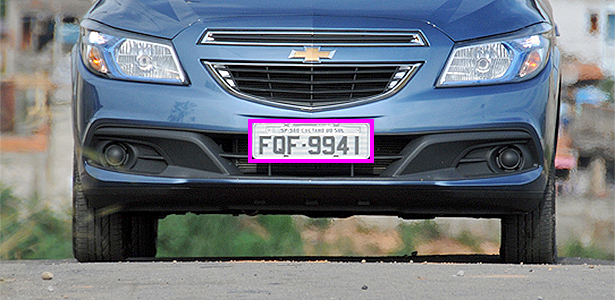
\includegraphics[scale=0.3]{img/carplaterec.png}
	\end{center}

	\end{itemize}
\end{frame}
\begin{frame}
	\frametitle{Segmentação de caracteres}
	\begin{itemize}
	\item Com a placa em mãos, o próximo passo é a \textbf{obtenção de cada 
	caractere separadamente};
	\item Para tanto, pode ser necessária uma etapa
	de pré-processamento, para normalizar a imagem, remover ruídos
	e acentuar características importantes;
	\item As projeções horizontal
	e vertical são técnicas muito utilizadas nesse processo.
	\end{itemize}
	
	\begin{figure}[!tbp]
		\centering
		\begin{minipage}[b]{.3\textwidth}
			
\includegraphics[scale=0.15]{img/F.jpg}
		\end{minipage}
		\begin{minipage}[b]{.3\textwidth}
			
\includegraphics[scale=0.15]{img/Q.jpg}
		\end{minipage}
	\end{figure}

\end{frame}
\begin{frame}
	\frametitle{Reconhecimento ótico de caracteres}
	\begin{itemize}
		\item Dado um caractere segmentado, resta \textbf{classificá-lo}
			em uma das 36 classes possíveis (26 letras + 10 dígitos);
		\item Entre as principais técnicas, as redes neurais e os
			classificadores estatísticos têm se destacado;
		\item Os resultados desta fase compõem a \textbf{saída do sistema}: um conjunto
			de caracteres ASCII correspondentes ao conteúdo
			da placa.
	\end{itemize}
	
	\begin{center}
	\Huge {\rmfamily F \qquad Q}
	\end{center}

\end{frame}

\subsection[Subsection]{Dados disponibilizados}
\begin{frame}
	\frametitle{Caracterização dos dados fornecidos}
	\begin{itemize}
		\item São caracteres já segmentados de imagens capturadas em 11 locais diferentes da UFRJ
			\cite{Allan};
		\item Cada classe (letra) possui aproximadamente 600 instâncias, ou seja,
			é garantido o \textbf{balanceamento};
		\item Os dados estão organizados
			em uma matriz $M_{11 \times 26}$ de vetores de \emph{structs} contendo os campos:
		\begin{description}
			\item [bmp\_data] Três matrizes iguais de dimensão $16 \times 16$, 
			representando a imagem do caractere  em tons de cinza;
			\item [target\_char] A classe à qual a imagem pertence;
			\item [target] O índice dessa classe;
			\item [local] Índice do local de origem. 
		\end{description}


	\end{itemize}
\end{frame}
\begin{frame}
	\frametitle{Separação das amostras}

	Para a tarefa de classificação, é importante a separação da massa de dados em 
	conjuntos de \textbf{treino}, \textbf{testes} e \textbf{validação}. Neste trabalho, foi
	escolhida a seguinte configuração de amostras: 

	\begin{table}[H]
	\centering
	\label{t:amostras}
		\begin{tabular}{c|c|c}
		Treino & Testes & Validação\\
		\hline
		60\% & 25\% & 15\%\\
		\end{tabular}
	\end{table}

	Para obtê-las, um \emph{script} em Octave/MATLAB foi criado,
	buscando garantir a \textbf{representatividade} quanto às letras
	e aos locais de obtenção.
\end{frame}

\subsection[Subsection]{Extração de descritores}
\begin{frame}
	\frametitle{Mapa de bits com projeções}
	A técnica adotada foi a de \textbf{mapa de bits com projeções}, a qual resulta em um vetor com os valores
	dos pixels normalizados mais as projeções horizontal
	e vertical, como resumido na tabela abaixo:

	\begin{table}[H]
	\resizebox{\textwidth}{!}{%
	\centering
	\label{t:descritores}
	\begin{tabular}{c|c|c|c}
	Descritores & Tipo & Valores & Passos da Extração\\
	\hline
	$N \times N$ pixels & Numérico & $[0,1]$ & Moldura, normalização, complemento\\
	Projeção horizontal ($N$) & Numérico & Inteiros & Binarização, soma das linhas\\
	Projeção vertical ($N$) & Numérico & Inteiros & Binarização, soma das colunas\\
	\end{tabular}
	}
	\end{table}
Neste caso, $N = 14$, totalizando \textbf{$\mathbf{224}$ descritores} à princípio.

\end{frame}

%%%%% Comentado %%%%%
\begin{comment}
\begin{frame}
	\frametitle{Passos para extração}
		\begin{enumerate}
			\item Retirada moldura branca presente em todas as imagens, reduzindo a dimensão para $14 \times 14$;
			\item Valores de 0 a 255 levados ao intervalo $[0,1]$, usando a função $im2double$;
			\item Obtenção do complemento da imagem, pela função $imcomplement$;
			\item Transformação da matriz de pixels $14 \times 14$ para vetor $1 \times 196$;
			\item Aplicada a função de binarização de Otsu, pelas funções $graythresh$ e $im2bw$;
			\item Somadas as linhas e as colunas da binarização, gerando, respectivamente,
		as projeções horizontal e a vertical;
			\item Concatenação das projeções ao vetor de pixels, gerando o vetor de descritores
		de dimensão $1 \times 224$.
		\end{enumerate}
\end{frame}
\end{comment}

\subsection[Subsection]{Análises estatísticas e tratamento
dos descritores}


\begin{frame}
	\frametitle{Conclusões sobre a análise de dados}
	\begin{itemize}
		\item A normalidade dos descritores, por não se fazer presente, não pode ser
		ferramenta imediata para a classificação;
		\item É possível reduzir a dimensionalidade do problema
		com base apenas na variância de certos descritores;
		\item A vizinhança dos pixels provoca uma maior correlação e,
		portanto, redundância de informação.
	\end{itemize}
\end{frame}


\section[Redução de dimensionalidade]{Redução de dimensionalidade}

\subsection[Redução por média e variância]{Redução por média e variância}
\begin{frame}
	\frametitle{Média e variância}
	\begin{itemize}
		\item Observou-se que 34 dos descritores ligados
		aos pixels possuem média abaixo de $10^{-2}$, o que
		pode indicar que são pixels de \emph{background};
		\item Desses, 29 possuem variância menor que $0.005$\footnote{A média das variâncias é 0.07}, mostrando
		que possuem baixa dispersão e que podem ser eliminados. Abaixo
		está uma representação deles:
	\end{itemize}
	
	\begin{center}
	\begin{figure}
		
\begin{tikzpicture}
			\draw[step=.2cm,gray,very thin] (-2,-2) grid (0.8,0.8);
			\fill[red!80!white] (-2,0.8) rectangle (0.8,0.6);
			\fill[orange!80!white] (-2,0.6) rectangle (-1.8,0.4);
			\fill[orange!80!white] (-0.6,0.6) rectangle (0.2,0.4);
			\fill[red!80!white] (0.6,0.6) rectangle (0.8,0.4);
			\fill[red!80!white] (-2,-1.8) rectangle (0.8,-2);
		\end{tikzpicture}
		\caption{\footnotesize Vermelho: variância $\leq 0.005$; Vermelho + Laranja: variância $\leq 0.01$}
	\end{figure}
	\end{center}
\end{frame}

\begin{frame}{Média e variância}
	Com isso, 29 descritores foram eliminados antes do uso de outros métodos de redução mais complexos, deixando-nos
	com \textbf{195 descritores}, a serem submetidos, nas próximas etapas, aos métodos de PCA, LDA e LPP.
\end{frame}


\subsection[PCA]{Principal Component Analysis}
\begin{frame}{PCA}

\begin{itemize}
	\item Analisando a representatividade dos autovalores, percebemos que 99\% da informação 
	seria mantida excluindo-se 93 descritores;
	\item Retiramos, então, as 93 primeiras colunas da matriz de autovetores $T$, obtendo a
	matriz de transformação $T'$, que operou sobre o conjunto de dados $D$, gerando a massa
	dados reduzida $D'$:
	$$D' = T'D$$
	\item Dessa forma, a partir do conjunto de 195 descritores, restaram-nos $\mathbf{102}$.
\end{itemize}
\end{frame}

\subsection[LDA]{Linear Discriminant Analysis}
\begin{frame}{LDA}

\begin{itemize}

	\item O LDA faz com que haja apenas C autovalores passíveis de consideração, pois
torna todos os outros nulos (ou muito próximos de 0); 
	\item Analisando-se os autovalores produzidos, notou-se que 24 deles concentravam 99\% da informação; 
	\item Assim, os 195 descritores foram reduzidos para apenas $\mathbf{24}$.

\end{itemize}
\end{frame}

\subsection[LPP]{Locality Preserving Projection}
\begin{frame}{LPP}
\begin{itemize}
	\item Neste trabalho, utilizou-se uma implementação em MATLAB disponível na Internet, a qual, 
	configurada para manter 99\% da informação, resultou em \textbf{30 descritores}.
\end{itemize}
\end{frame}

\subsection[Resumo]{Resumo}
\begin{frame}{Resumo}
	Por média e variância: $224 \to 195$\\~\\
	Em seguida:\\
	\begin{center}
	\begin{tabular}{c | l}
		Método 		& Quantidade		\\
		\hline
		PCA 		& $195 \to 102$		\\
		LDA 		& $195 \to 24$ 		\\
		LPP 		& $195 \to 30$ 		\\ 
	\end{tabular}
	\end{center}
\end{frame}


\section[Classificação]{Classificação}

\subsection[Metodologia de testes]{Metodologia de testes}
\begin{frame}{Testes}
	\begin{itemize}
		\item Conjunto de testes dividido em 30 subconjuntos de 121 instâncias;
		\item Cada classificador foi testado com os $N = 30$ subconjuntos, gerando
		      30 medições, cuja média denotamos por $\mu$;
		\item Com a média, calculamos a margem de erro $E$ com $\alpha = 0.05$ seguindo a fórmula:
		      $$E= Z_{\frac{\alpha}{2}}\times\frac{\sigma}{\sqrt{N}}$$	
		      E expressamos o intervalo de confiança na forma
		      $$\mu \pm E.$$
	\end{itemize}
\end{frame}

\subsection[MLP]{Multilayer Perceptron}

\begin{frame}{Representação do target para MLP}

Para a MLP, representamos o target como um vetor binário
de 26 posições, contendo o valor 1 apenas na posição
correspondente ao número da classe.\\~\\

Por exemplo, representamos a letra \textbf{A} por
$$[1 0 0 0 0 0 0 0 0 0 0 0 0 0 0 0 0 0 0 0 0 0 0 0 0 0]$$

\end{frame}

\begin{frame}{Arquitetura e criação}
	Utilizamos uma rede com \textbf{duas camadas}, sendo a escondida
	com um número variado de neurônios e a de saída com 26, o tamanho
	do vetor de \emph{target}.\\~\\

	Para criar, usamos, no MATLAB, as funções:

\begin{description}
        \item [patternnet] Recebe a quantidade de neurônios artificiais
                da camada escondida, retornando um objeto correspondente
                à configuração da rede neural. 
        \item [train] Utiliza o objeto construído com a \emph{patternnet} para
                treinar a rede neural segundo os parâmetros definidos. 
\end{description}
\end{frame}

\begin{frame}{Parâmetros fixos}

Os seguintes parâmetros da arquitetura e do treino
 das redes foram fixados:

\begin{table}[H] 
\centering 
\begin{tabular}{c|r} 
        Parâmetro & Valor \\ 
        \hline 
        trainParam.epochs & 1000\\ 
        trainParam.goal & 0.001\\ 
        performFcn & mse\\ 
        trainParam.max\_fail & 50\\ 
        trainParam.min\_grad & $1 \times 10^{-8}$\\ 
        divideFcn & dividerand\\ 
        trainFcn & trainrp\\ 
\end{tabular} 
%\caption{Parâmetros fixos para as redes MLP treinadas neste trabalho.} 
%\label{tab:fixmlp} 
\end{table}


\end{frame}

\begin{frame}{Parâmetros variados}

	\begin{block}{Número de neurônios}
		O número inicial de neurônios na camada escondida 
			foi determinado pelo cálculo:
			$$N_{hidden} = \frac{N_{descritores} + N_{saida}}{2}$$			
		Depois, somamos 10, 20 e 30 a esse número, gerando quatro quantidades.
	\end{block}

	\begin{block}{Funções de propagação}
		Testamos combinações das funções tansig, logsig e linear.
	\end{block}

\end{frame}

\begin{frame}{Parâmetros variados}
	Em resumo:
	\begin{table}[H] 
		\centering 
		\begin{tabular}{c|r} 
			Parâmetro & Valor \\ 
			\hline 
			propagação da escondida 	& tansig, logsig\\
			propagação da saída 	        & tansig, linear, logsig\\
			número de neurônios		& $N$, $N+10$, $N+20$, $N+30$\\
		\end{tabular} 
		%\caption{Parâmetros fixos para as redes MLP treinadas neste trabalho.} 
		%\label{tab:fixmlp} 
	\end{table}
\end{frame}

\begin{frame}{Condições de parada}
	
Analisamos três condições de parada:

	\begin{block}{Epochs}
        Quando a quantidade de ciclos ultrapassa
                um limite;
	\end{block}

	\begin{block}{Checagens de Validação}
        	Quando o erro relativo ao conjunto
                de validação atinge certo número de não descrescimentos consecutivos;
	\end{block}
	
	\begin{block}{Gradiente}
		Quando o gradiente do erro diminui mais que
                um limite determinado.
	\end{block}

\end{frame}

\begin{frame}{Testes com logsig na saída}
	
	Os testes com logsig na camada de saída não lograram êxito, 
	pois terminavam em cerca de 4 ciclos e apresentavam desempenho
	inferior a 5\%.\\~\\

	Por essa razão, descartamos essa função nessa camada. \\~\\

	Quando colocada na camada escondida, entretanto, apresentou
	resultados satisfatórios, como exibido nas próximas seções.

\end{frame}


\begin{frame}{Resultados com PCA}
	\footnotesize
        \begin{tabularx}{\linewidth}{| c | c | c | c | c | c | c |}
                \toprule
                TRD & Escondida & Saída & Neurônios & Epochs & MP & ACC $\pm$ ME\\
                \midrule
                \endhead
                \multirow{16}{*}{PCA} & \multirow{8}{*}{tansig} & \multirow{4}{*}{purelin} & 64 & 1000 & E & $95.44\% \pm 3.03\%$\\
                                      &                         &                          & 74 & 1000 & E & $95.27\% \pm 3.01\%$\\
                                      &                         &                          & 84 & 1000 & E & $95.99\% \pm 3.03\%$\\
                                      &                         &                          & 94 & 1000 & E & $95.33\% \pm 3.01\%$\\\cline{3-7}
                                      &                         & \multirow{4}{*}{tansig}  & 64 & 157 & V & $97.27\% \pm 3.11\%$\\*
                                      &                         &                          & 74 & 141 & V & $96.52\% \pm 3.11\%$\\*
                                      &                         &                          & 84 & 151 & V & $97.30\% \pm 3.03\%$\\*
                                      &                         &                          & 94 & 135 & V & $96.97\% \pm 3.09\%$\\\cline{2-7}
                                      & \multirow{8}{*}{logsig} & \multirow{4}{*}{purelin} & 64 & 1000 & E & $96.86\% \pm 3.14\%$\\*
                                      &                         &                          & 74 & 1000 & E & $97.30\% \pm 3.11\%$\\*
                                      &                         &                          & 84 & 1000 & E & $97.00\% \pm 3.06\%$\\*
                                      &                         &                          & 94 & 1000 & E & $97.66\% \pm 3.06\%$\\*\cline{3-7}
                                      &                         & \multirow{4}{*}{tansig}  & 64 & 182 & V & $97.11\% \pm 3.09\%$\\
                                      &                         &                          & 74 & 162 & V & $97.58\% \pm 3.09\%$\\
                                      &                         &                          & 84 & 169 & V & $96.41\% \pm 3.09\%$\\
                                      &                         &                          & 94 & 126 & V & $97.36\% \pm 3.01\%$\\
                \bottomrule
                %\caption{Resultados do classificador MLP para dados tratados por PCA.}
                %\label{tab:mlppca}
        \end{tabularx}
\end{frame}

\begin{frame}{Resultados com LDA}
	\footnotesize
        \begin{tabularx}{\linewidth}{| c | c | c | c | c | c | c |}
                \toprule
                TRD & Escondida & Saída & Neurônios & Epochs & MP & ACC $\pm$ ME\\
                \midrule
                \endhead

                \multirow{16}{*}{LDA} & \multirow{8}{*}{tansig} & \multirow{4}{*}{purelin} & 25 & 1000 & E & $ 64.88\% \pm 2.05\%$\\
                                      &                         &                          & 35 & 1000 & E & $ 67.11\% \pm 2.14\%$\\
                                      &                         &                          & 45 & 1000 & E & $ 69.02\% \pm 2.08\%$\\
                                      &                         &                          & 55 & 1000 & E & $ 70.77\% \pm 2.11\%$\\\cline{3-7}
                                      &                         & \multirow{4}{*}{tansig}  & 25 & 649 & V & $ 72.13\% \pm 2.11\%$\\
                                      &                         &                          & 35 & 461 & V & $ 75.05\% \pm 2.27\%$\\
                                      &                         &                          & 45 & 652 & V & $ 74.44\% \pm 2.27\%$\\
                                      &                         &                          & 55 & 315 & V & $ 74.63\% \pm 2.27\%$\\\cline{2-7}
                                      & \multirow{8}{*}{logsig} & \multirow{4}{*}{purelin} & 25 & 1000 & E & $ 63.09\% \pm 1.76\%$\\
                                      &                         &                          & 35 & 1000 & E & $ 68.38\% \pm 2.11\%$\\
                                      &                         &                          & 45 & 1000 & E & $ 70.16\% \pm 2.06\%$\\
                                      &                         &                          & 55 & 1000 & E & $ 71.97\% \pm 2.06\%$\\*\cline{3-7}
                                      &                         & \multirow{4}{*}{tansig}  & 25 & 390 & V & $ 73.22\% \pm 2.25\%$\\
                                      &                         &                          & 35 & 360 & V & $ 74.72\% \pm 2.35\%$\\
                                      &                         &                          & 45 & 200 & V & $ 74.99\% \pm 2.41\%$\\
                                      &                         &                          & 55 & 280 & V & $ 75.14\% \pm 2.11\%$\\
                \bottomrule
                %\caption{Resultados do classificador MLP para dados tratados por LDA.}
                %\label{tab:mlplda}
        \end{tabularx}
\end{frame}

\begin{frame}{Resultados com LPP}
	\footnotesize
	\begin{tabularx}{\linewidth}{| c | c | c | c | c | c | c |}
                \toprule
                TRD & Escondida & Saída & Neurônios & Epochs & MP & ACC $\pm$ ME\\
                \midrule
                \endhead
                \multirow{16}{*}{LPP} & \multirow{8}{*}{tansig} & \multirow{4}{*}{purelin} & 28 & 1000 & E & $ 89.86\% \pm 2.84\%$\\
                                      &                         &                          & 38 & 1000 & E & $ 90.74\% \pm 2.90\%$\\
                                      &                         &                          & 48 & 1000 & E & $ 92.41\% \pm 2.90\%$\\
                                      &                         &                          & 58 & 1000 & E & $ 92.77\% \pm 2.84\%$\\\cline{3-7}
                                      &                         & \multirow{4}{*}{tansig}  & 28 & 433 & V & $ 96.16\% \pm 3.11\% $\\*
                                      &                         &                          & 38 & 388 & V & $ 96.86\% \pm 3.11\% $\\*
                                      &                         &                          & 48 & 320 & V & $ 96.44\% \pm 3.09\% $\\*
                                      &                         &                          & 58 & 240 & V & $ 96.94\% \pm 3.09\% $\\\cline{2-7}
                                      & \multirow{8}{*}{logsig} & \multirow{4}{*}{purelin} & 28 & 1000 & E & $ 91.32\% \pm 2.84\%$\\
                                      &                         &                          & 38 & 1000 & E & $ 93.55\% \pm 2.95\%$\\
                                      &                         &                          & 48 & 1000 & E & $ 93.08\% \pm 2.90\%$\\
                                      &                         &                          & 58 & 1000 & E & $ 94.58\% \pm 3.06\%$\\\cline{3-7}
                                      &                         & \multirow{4}{*}{tansig}  & 28 & 400 & V & $ 96.75\% \pm 3.03\%$\\
                                      &                         &                          & 38 & 246 & V & $ 96.77\% \pm 3.09\%$\\
                                      &                         &                          & 48 & 346 & V & $ 96.74\% \pm 3.11\%$\\
                                      &                         &                          & 58 & 369 & V & $ 96.55\% \pm 3.09\%$\\
                \bottomrule
                %\caption{Resultados do classificador MLP para dados tratados por LPP.}
                %\label{tab:mlplpp}
        \end{tabularx}
\end{frame}

\begin{frame}{Análises}
	\begin{itemize}
		\item De imediato, nota-se que o método LDA não gerou
		bons resultados em comparação aos demais;
		\item A técnica PCA gerou os melhores resultados, ainda que não tão distantes do LPP;
		\item A quantidade de neurônios não pareceu influenciar consideravelmente nas
		acurácias;
		\item Essa semelhança de desempenho do PCA com LPP
indica que, caso se necessite economizar recursos de tempo e espaço, o LPP pode ser
uma alternativa eficaz, já que gerou menos descritores e, consequentemente, necessitou de
menos neurônios.
		\item Com isso, conclui-se que as redes MLP são, de fato, classificadores com desempenho 
satisfatório na tarefa de reconhecimento óptico de caracteres de placas.
	\end{itemize}
\end{frame}

\subsection[SVM]{Support Vector Machine}

\begin{frame}{Implementação utilizada}

\end{frame}
